\hypertarget{confidence-in-communities}{\section{Confidence in
communities}\label{confidence-in-communities}}

\protect\hyperlink{confidence-in-communities}{}

\subsection{Statistical significance}\label{statistical-significance}

Although it is counterintuitive, completely random graphs, when viewed a
certain way, can be seen to have community structure. In a random graph,
known as an Erdős--Rényi graph \autocite{erdos_evolution_1960}, every
node has an equal probability of being linked to every other node.
Fig.~\ref{fig:randomcommunities} shows how a random graph can show group
structure. The top left shows the adjacency matrix of a random graph
with nodes in arbitrary order; this looks like random white noise. By
rearranging the order of the nodes in the same random graph, as in the
other panes of the figure, a community structure becomes apparent. This
is not actual community structure we are interested in, but rather
artifacts of the randomness. Nevertheless, community detection methods
can pick up on them and find artificial structure in what should be
random. These effects are even more pronounced for sparse graphs, a
category which includes most real-world networks we would like to
analyze \autocite{fortunato_community_2016}.

\begin{figure}
\centering
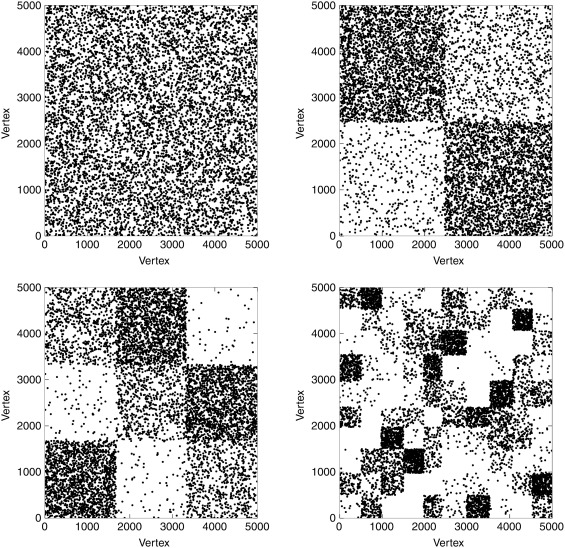
\includegraphics{img/fortunato2016_fig29_randomcommunities.jpg}
\caption{Artificial community structure in a random graph. Each of the
four graphs represent the adjacency matrix of the same 5000-node random
graph, in which every pair of nodes has equal probility of sharing a
link. The top right matrix shows the nodes in arbitrary order, and the
impression is one of random white noise. The others are simply
rearrangements of the nodes for the same random graph. A community
structure can be seen from what is actually random fluctuations in the
network construction process. Figure from
\autocite{fortunato_community_2016}.}\label{fig:randomcommunities}
\end{figure}

This raises the question: how can we be confident that the communities
detected by an algorithm reflect actual community structure, and not an
artifact of random noise? This is an open problem in network science,
but several attempts have been made to address it.

One approach is to compare the results to an appropriate null model. The
most popular null model has been the configuration model, which can
generate any configuration of a network given a number of nodes, number
of edges, and degree sequence for every node. One can use an ensemble of
these networks and compare them against empirical results. Any measure
of the graph, for example a centrality measure of a given node, can be
compared with the same measure on a number of generated null models; a
\(p\)-value can then be calculated as the fraction of model
configurations that yield the same value for the measure as the observed
network \autocite{fortunato_community_2016}. (It may be difficult to
operationalize ``same value'' here---requiring an exact match might make
this test too insensitive, but allowing for variation would introduce
more noise.) One could apply this approach to the community structure as
a whole, or to individual communities, or to community membership of
individual nodes, measuring these phenomena against their presence in an
ensemble of generated graphs.

Another approach is to consider the robustness of a given network to
perturbations in the network structure. From a conceptual standpoint,
this approach differs from the above one in that it does not consider
the network structure as having been generated from a stochastic
process, and attempt to model that process. Rather, it takes the
structure as given and observes the effects of random noise introduced
into this structure on the communities that are detected. This approach
has the advantages that it is applicable to any method, and it is not
restricted to a particular null model
\autocites{rosvall_mapping_2010}{mirshahvalad_significant_2012}.\footnote{In
  practice, however, a particular null model is often implied in a
  perturbation strategy, as can be seen in the discussed examples.}

Several strategies for perturbing networks have been proposed. Gfeller
et al. \autocite{gfeller_finding_2005} employ a strategy on weighted
graphs in which edge weights are increased or decreased by a relative
amount \(0 < \delta < 1\). After choosing \(\delta\), multiple
realizations of the graph are clustered using any method, and the
\emph{in-cluster} probability of each pair of adjacent vertices
\(p_{ij}\) is calculated as the fraction of realizations in which they
were clustered together. Edges with \(p_{ij} < \theta\) are considered
to be \emph{external} edges. This approach has as a weakness the need to
choose values for \(\delta\) and \(\theta\). The authors also provide a
way to measure the overall stability of the partition using these
in-cluster probabilities; this measure needs to be compared against a
null model.

Karrer et al. \autocite{karrer_robustness_2008} use a strategy for
unweighted graphs of network rewiring. Each edge is considered and
either left alone or, with probability \(\alpha\), it is removed and
replaced with another edge between a pair of vertices \((i, j)\) chosen
at random with probability \(p_{ij} = k_i k_j / 2m\) (\(k_i\) and
\(k_j\) are the degrees of \(i\) and \(j\); \(m\) is the number of edges
in the graph). This probability is the same one used in the null model
of modularity. The authors generated multiple graphs for different
values of \(\alpha\), and compared their clusterings to each other using
the variation of information \(V\). They then plotted \(V\) against
\(\alpha\) to see how different levels of perturbation would affect the
stability of the network structure. They compared the function
\(V(\alpha)\) against a null model---again, the null model of
modularity.

Rosvall and Bergstrom use a parametric bootstrap resampling method to
measure significance of communities. To resample the graph, each edge is
assigned a weight from a Poisson distribution with mean equal to the
original edge weight. The authors then cluster both the original and
resampled networks (any clustering method can be used; the authors used
Infomap). Each cluster of the original graph is considered, and of these
nodes the largest subset clustered in the same group in at least 95\% of
the resampled networks is deemed a significant cluster. By applying this
technique on citation graphs at different time points, the authors track
the change in the community structure over time (see subsection
``\protect\hyperlink{networks-of-scholarship}{Networks of scholarship}''
in section ``\protect\hyperlink{applications}{Applications of community
detection}'')

Mirshahvalad et al. \autocite{mirshahvalad_significant_2012} propose a
\emph{constructive} perturbation approach suitable for sparse networks.
These networks have a danger that communities can be ``shattered'' into
small modules if there are missing links due to noise in the data.
\emph{Link prediction} is employed to add links to the network,
strengthening the communities. The link prediction strategy used is
triangle completion, in which a fraction of open triangles are completed
by adding a link. This is a relatively simple strategy, and more
sophisticated methods can be used, but the authors show that it performs
well on benchmark graphs that have been shattered. This method can be
used as a bootstrap resampling technique, and significance can be
measured based on the resampled distribution. A weakness of this method
is that the number of links to be added needs to be chosen, but the
benchmark experiments suggest that results are robust to this choice.

In summary, measuring our confidence in community detection techniques
seems to be a hard problem. Network data are highly interrelated, so
typical independence assumptions that underlie many statistical methods
do not apply. One important issue is the lack of a realistic null model.
Typical null models assume that any node can be connected to any other
with equal probability, but this assumption does not intuitively hold
for large networks. More appropriate would be to have a ``horizon'' of
nodes that each node is more likely to interact with, but such horizons
have yet to be defined \autocite{fortunato_community_2010}. The lack of
appropriate null models is a problem for generative models that rely on
them explicitly, but they tend to underlie assumptions behind link
perturbation and resampling strategies as well. More work remains to be
done to arrive at standard ways of measuring our confidence in the
results of community detection.

\subsection{Algorithmic inaccuracy}\label{algorithmic-inaccuracy}

Our confidence in the performance of a given algorithm due to, for
instance, using different random seeds is a distinct issue. The
statistical significance of community detection is a question of
confidence in the \emph{theory} behind our method. Variation in the
results due to the fact that we are necessarily using approximating
algorithms (due to the complexity of the problem), on the other hand,
affects our confidence in the \emph{implementation} of our method. In
the case of Infomap, during each pass of the core algorithm, the nodes
are considered one at a time in random order, and merged with one of its
neighbors in order to give maximum improvement to the objective function
(the map equation). In principle, there should be one global minimum for
the map equation, corresponding to the one optimal community structure.
In practice, it does seem like the order that the nodes are considered
does make a difference in the final value of the map equation---i.e.,
how well Infomap is able to approximate this global optimum. For
example, in a recent experiment in which I performed 106 runs of Infomap
on the JSTOR article citation network, I found an approximately normal
distribution of final values between 11.334 and 11.364 (mean 11.348,
standard dev 0.00577). These numbers are of course difficult to
interpret, but they do show that there is at least some variation.

The Infomap algorithm is based on the Louvain method for modularity
maximization. In the paper introducing the Louvain method, Blondel el
al. report on this issue. While they see the same type of variation in
relation to the random order, they claim the effect is small, and they
are more concerned with the effect the order has on computation time.
They leave further understanding of the issue to future study
\autocite{blondel_fast_2008}.

In light of this, it would not be a bad idea for someone using any
approximating method to perform multiple runs if she is interested in
finding the best solution possible. More work is needed to understand
specifically the effect of the random seed on the performance of
Infomap.
